\documentclass{beamer}
\usetheme{default}
\setbeamertemplate{navigation symbols}{}

\title{Ronald: A Multithreaded Path Tracing Renderer}
\subtitle{SENG 475 Final Project}
\author{Jayden Chan}
\institute{\href{https://github.com/jayden-chan/ronald}{https://github.com/jayden-chan/ronald}}
\date{August 15 2022}

\begin{document}

\begin{frame}
\titlepage
\end{frame}

\begin{frame}{What is Path Tracing?}
    \begin{itemize}[<+->]
        \item Computer graphics technique for creating photo realistic renderings
        \item Monte Carlo integration
        \item Based on the physical characteristics of light and the world (PBR)
        \item Very slow
    \end{itemize}
\end{frame}

\begin{frame}{What is Path Tracing?}
    \begin{center}
        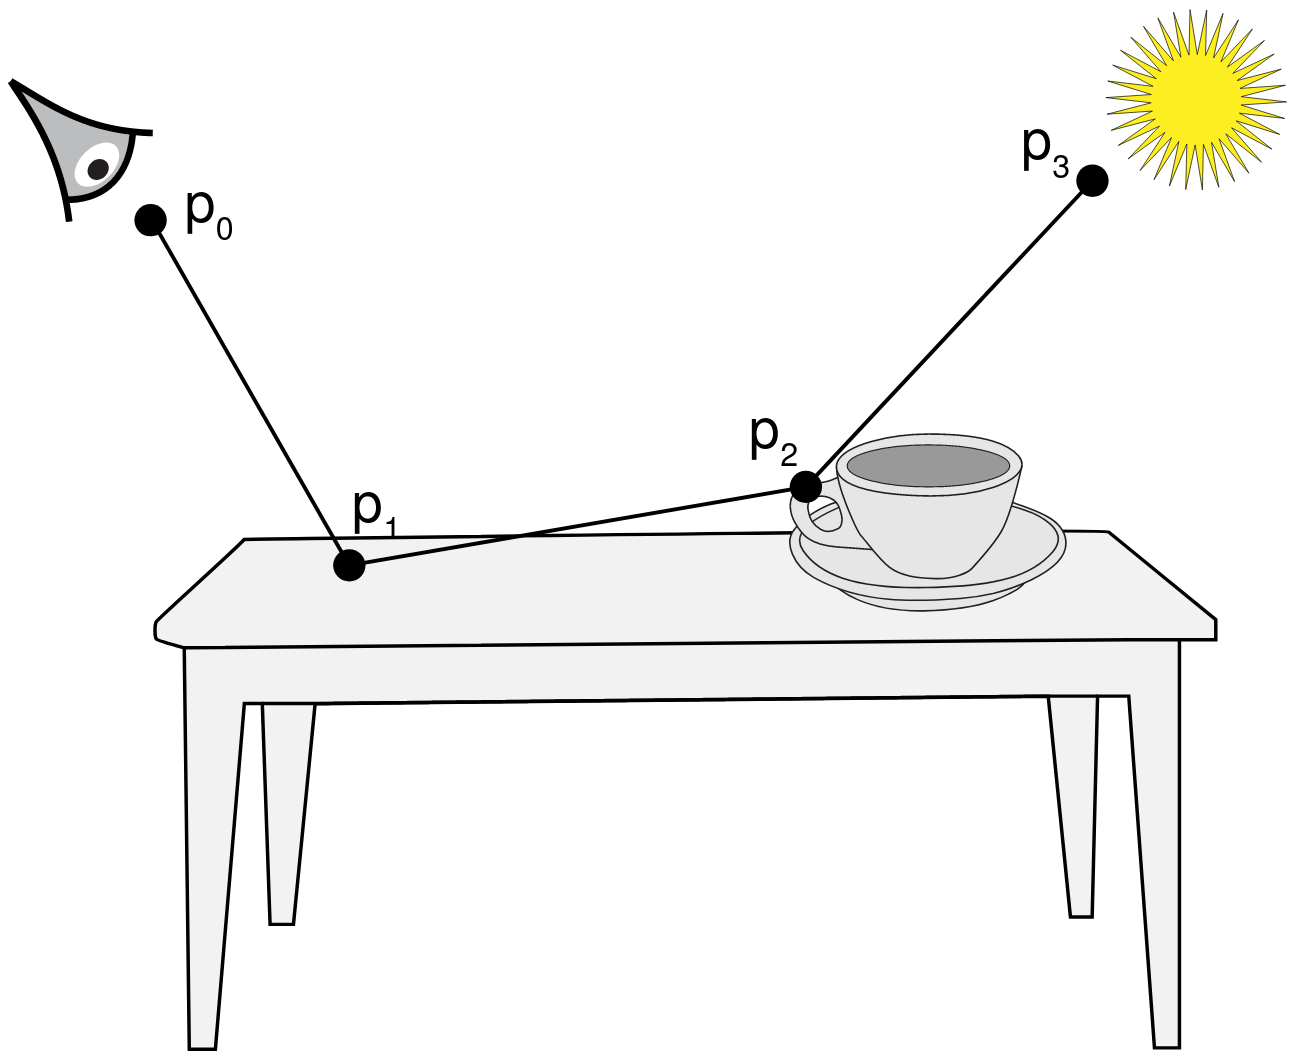
\includegraphics[width=0.9\textwidth]{./path_tracing.png}
    \end{center}
\end{frame}

\begin{frame}{What is Path Tracing? -- The Rendering Equation}
    \begin{center}
        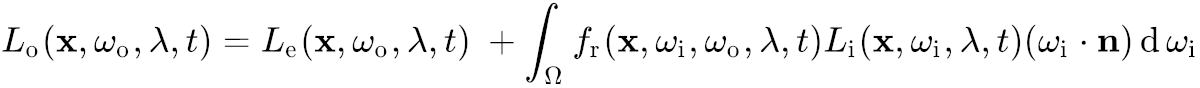
\includegraphics[width=1.0\textwidth]{./rendering-eq.png}
    \end{center}
\end{frame}

\begin{frame}{Industrial Path Tracers}
    \begin{center}
    
\includegraphics[width=0.5\textwidth]{./renderman.png}\\
    \vspace{0.2cm}
    
\includegraphics[width=0.5\textwidth]{./arnold.png}\\
    
\includegraphics[width=0.5\textwidth]{./blender.png}\\
    
\includegraphics[width=0.5\textwidth]{./octane.png}\\
    
\includegraphics[width=0.2\textwidth]{./povray.png}
    \end{center}
\end{frame}

\begin{frame}{Industrial Path Tracers}
    
\includegraphics[width=0.2\textwidth]{./renderman.png}
    \begin{center}
    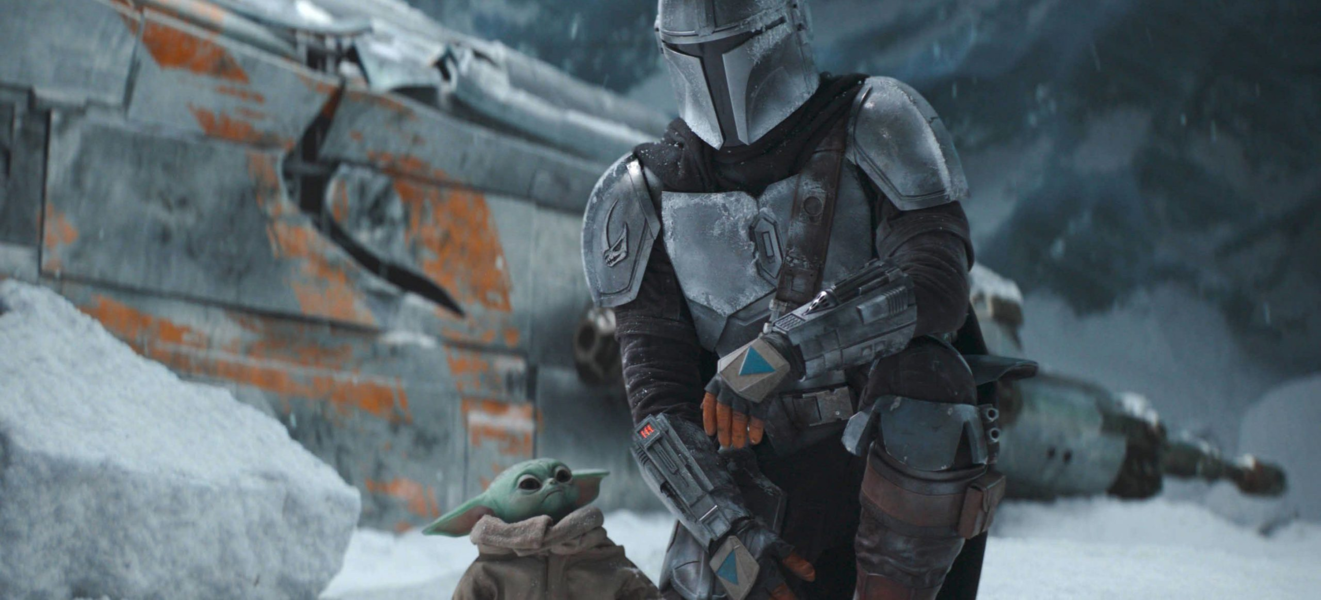
\includegraphics[width=1.0\textwidth]{./renderman-2.png}
    \end{center}
\end{frame}

\begin{frame}{The Cornell Box}
    POVRay rendering of the famous Cornell Box scene
    \begin{center}
        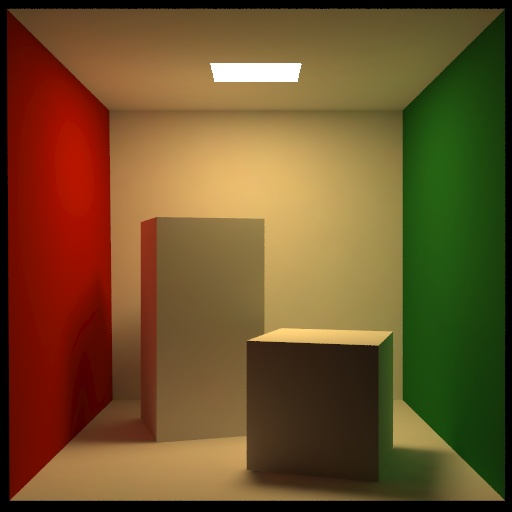
\includegraphics[width=0.65\textwidth]{../img/povray.jpg}
    \end{center}
\end{frame}

\begin{frame}{The Cornell Box}
    Left: POVRay reference render\\
    Right: My rendering
    \begin{center}
        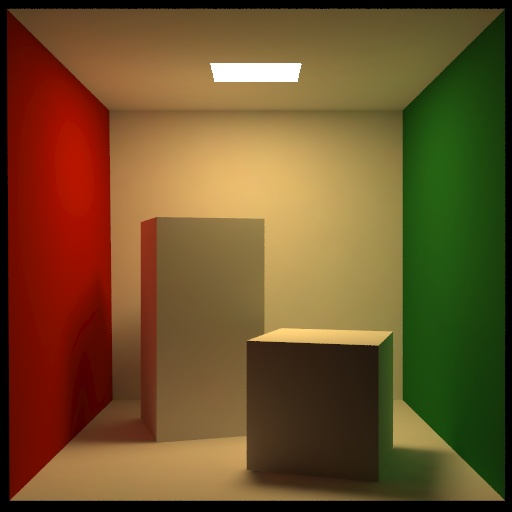
\includegraphics[width=0.45\textwidth]{../img/povray.jpg}
        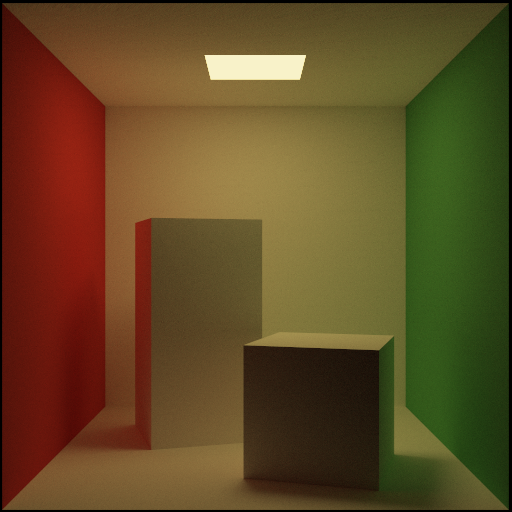
\includegraphics[width=0.45\textwidth]{../img/cornell_4.png}
    \end{center}
\end{frame}

\begin{frame}{Example: Monte Carlo Integration Convergence}
    Samples: 45000
    \begin{center}
        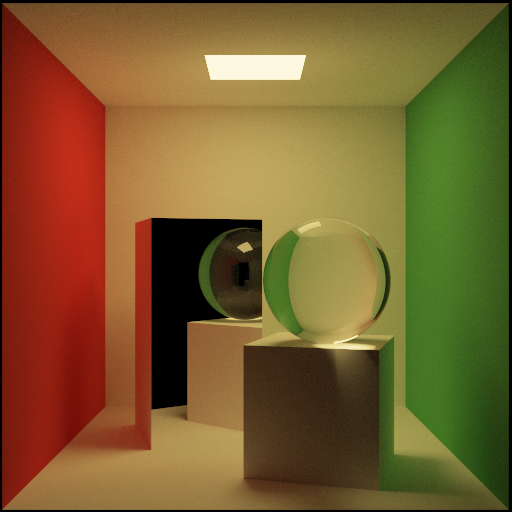
\includegraphics[width=0.65\textwidth]{../img/convergence/cornell-45000.png}
    \end{center}
\end{frame}

\begin{frame}{Example: Monte Carlo Integration Convergence}
    Samples: 10
    \begin{center}
        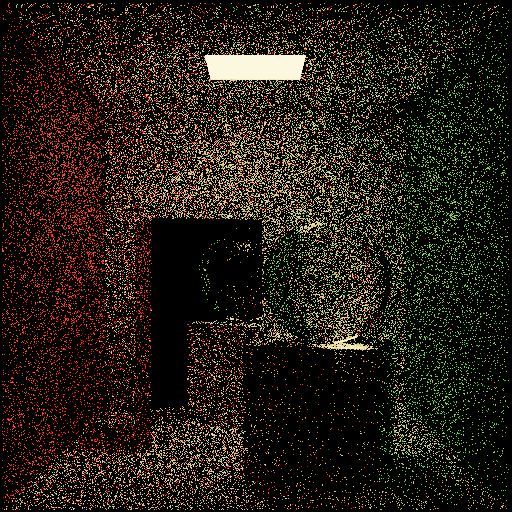
\includegraphics[width=0.65\textwidth]{../img/convergence/cornell-00010.png}
    \end{center}
\end{frame}

\begin{frame}{Example: Monte Carlo Integration Convergence}
    Samples: 25
    \begin{center}
        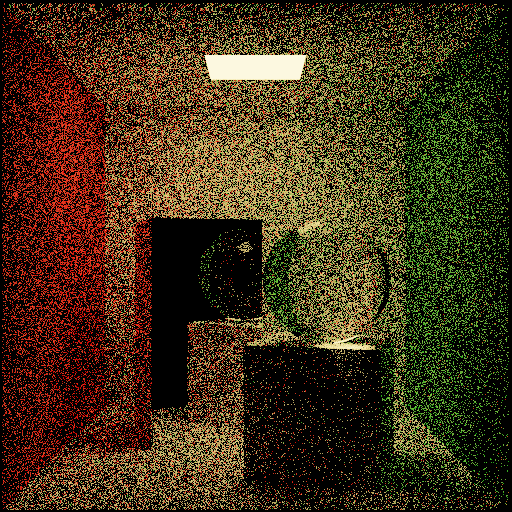
\includegraphics[width=0.65\textwidth]{../img/convergence/cornell-00025.png}
    \end{center}
\end{frame}

\begin{frame}{Example: Monte Carlo Integration Convergence}
    Samples: 50
    \begin{center}
        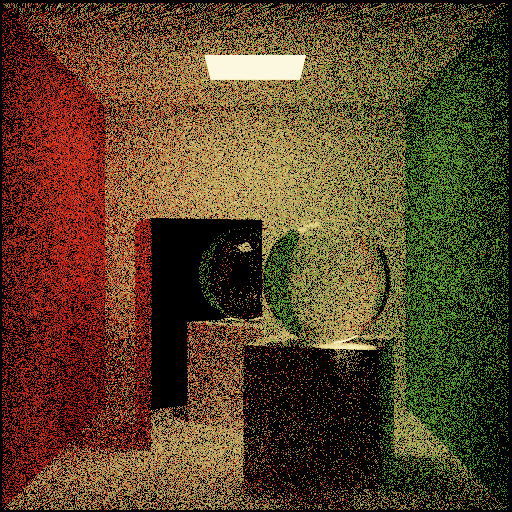
\includegraphics[width=0.65\textwidth]{../img/convergence/cornell-00050.png}
    \end{center}
\end{frame}

\begin{frame}{Example: Monte Carlo Integration Convergence}
    Samples: 100
    \begin{center}
        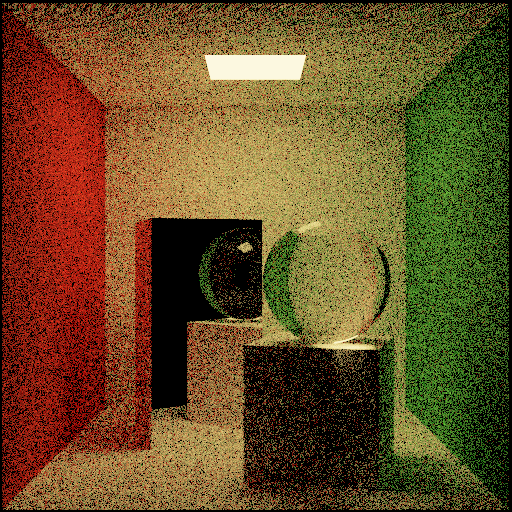
\includegraphics[width=0.65\textwidth]{../img/convergence/cornell-00100.png}
    \end{center}
\end{frame}

\begin{frame}{Example: Monte Carlo Integration Convergence}
    Samples: 200
    \begin{center}
        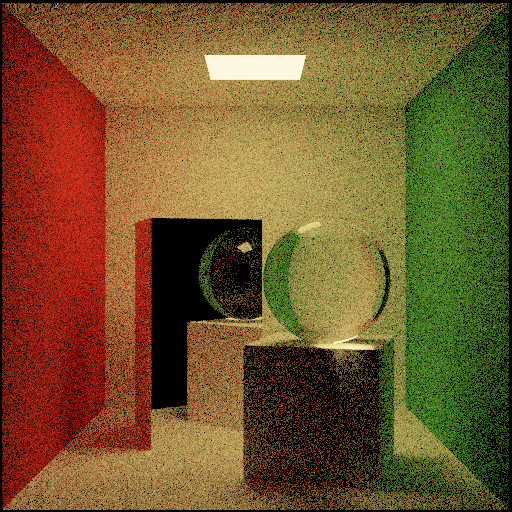
\includegraphics[width=0.65\textwidth]{../img/convergence/cornell-00200.png}
    \end{center}
\end{frame}

\begin{frame}{Example: Monte Carlo Integration Convergence}
    Samples: 500
    \begin{center}
        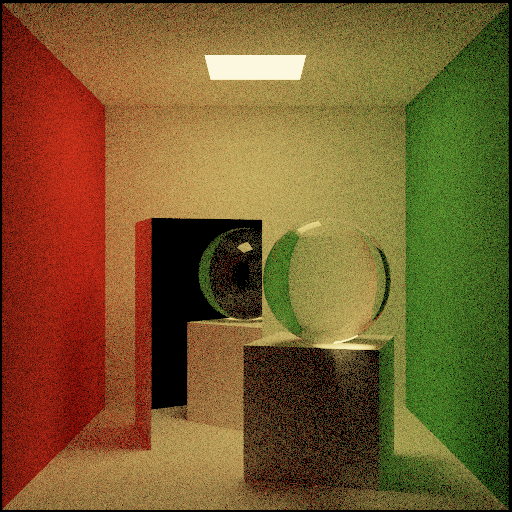
\includegraphics[width=0.65\textwidth]{../img/convergence/cornell-00500.png}
    \end{center}
\end{frame}

\begin{frame}{Example: Monte Carlo Integration Convergence}
    Samples: 1300
    \begin{center}
        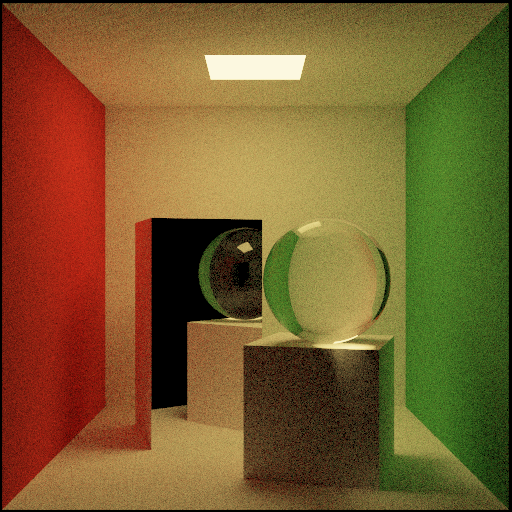
\includegraphics[width=0.65\textwidth]{../img/convergence/cornell-01300.png}
    \end{center}
\end{frame}

\begin{frame}{Example: Monte Carlo Integration Convergence}
    Samples: 3000
    \begin{center}
        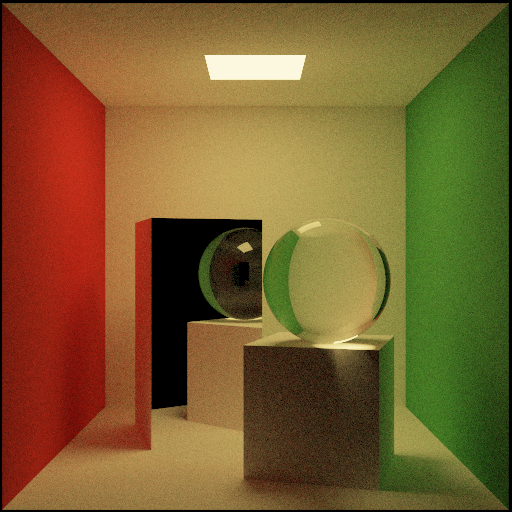
\includegraphics[width=0.65\textwidth]{../img/convergence/cornell-03000.png}
    \end{center}
\end{frame}

\begin{frame}{Example: Monte Carlo Integration Convergence}
    Samples: 15000
    \begin{center}
        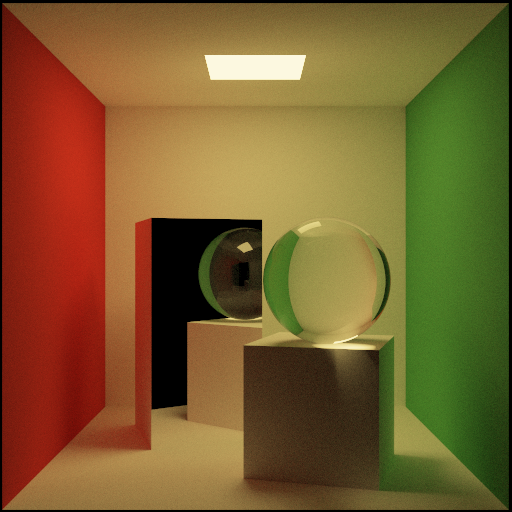
\includegraphics[width=0.65\textwidth]{../img/convergence/cornell-15000.png}
    \end{center}
\end{frame}

\begin{frame}{Example: Monte Carlo Integration Convergence}
    Samples: 45000
    \begin{center}
        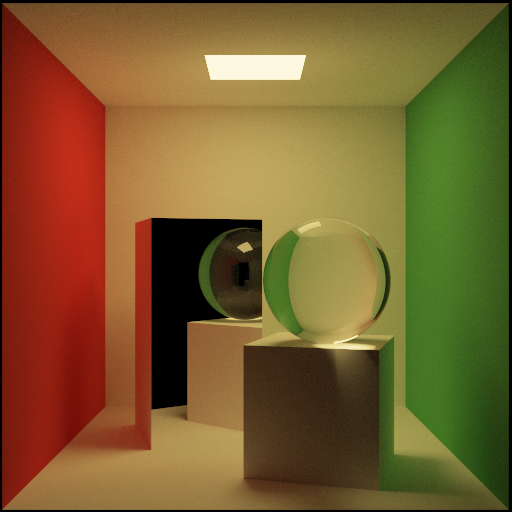
\includegraphics[width=0.65\textwidth]{../img/convergence/cornell-45000.png}
    \end{center}
\end{frame}

\begin{frame}{Showcase: Spheres and Mirrors}
    \footnotesize{
    Samples: 24000\\
    Resolution: 874x512\\
    Scene file: \texttt{../tests/scenes/spheres.jsonc}
    }
    \begin{center}
        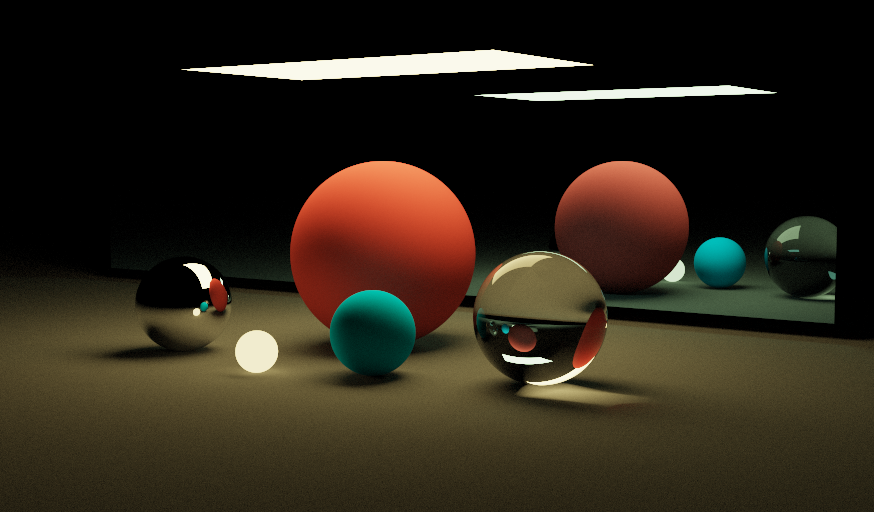
\includegraphics[width=1.00\textwidth]{../img/spheres.png}
    \end{center}
\end{frame}

\begin{frame}{Showcase: Spheres and Mirrors (Zoomed)}
    \footnotesize{
    Samples: 16000\\
    Resolution: 874x512\\
    Scene file: \texttt{../tests/scenes/spheres.jsonc}
    }
    \begin{center}
        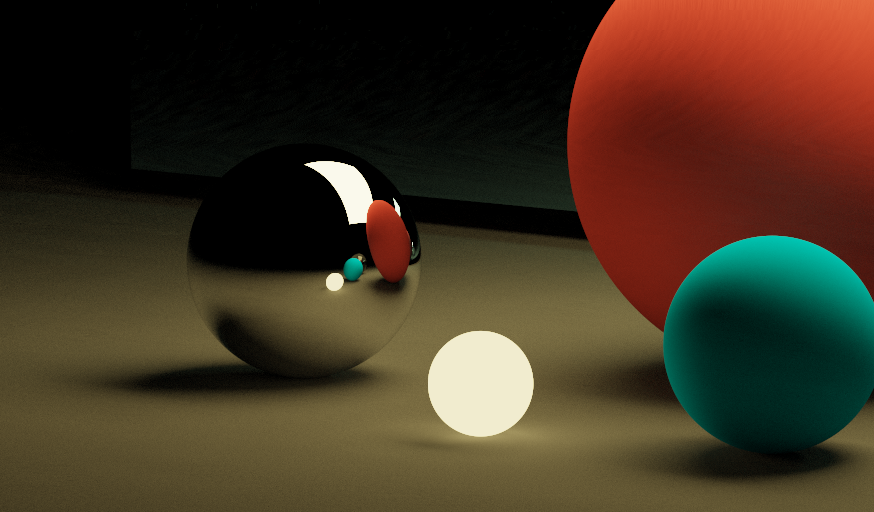
\includegraphics[width=1.00\textwidth]{../img/spheres-2.png}
    \end{center}
\end{frame}

\begin{frame}{Showcase: Suzanne Test Model}
    \footnotesize{
    Samples: 4000\\
    Resolution: 512x512\\
    Scene file: \texttt{../tests/scenes/monkey\_front.jsonc}
    }
    \begin{center}
        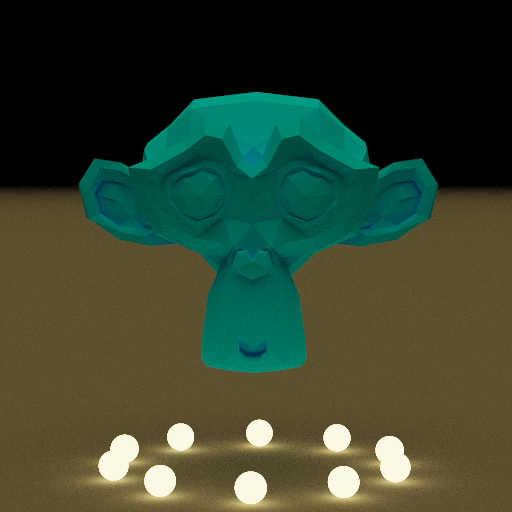
\includegraphics[width=0.65\textwidth]{../img/suzanne_blue.png}
    \end{center}
\end{frame}

\begin{frame}{Showcase: Suzanne Test Model in Glass}
    \footnotesize{
    Samples: 15000\\
    Resolution: 512x512\\
    Scene file: \texttt{../tests/scenes/monkey.jsonc}
    }
    \begin{center}
        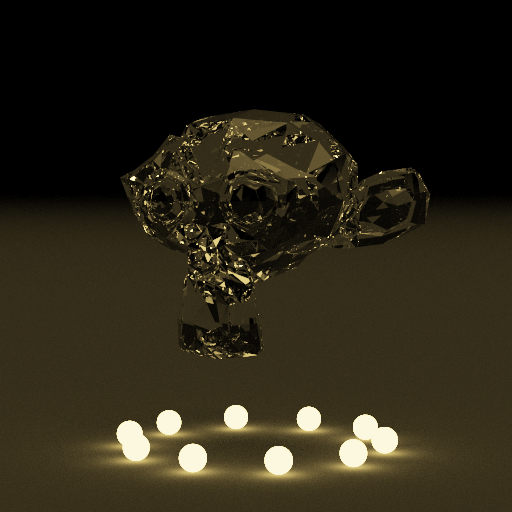
\includegraphics[width=0.65\textwidth]{../img/suzanne_glass.png}
    \end{center}
\end{frame}

\begin{frame}{Showcase: Camera Aperture}
    \footnotesize{
    Samples: 32000\\
    Resolution: 512x512\\
    Scene file: \texttt{../tests/scenes/spheres\_dof.jsonc}
    }
    \begin{center}
        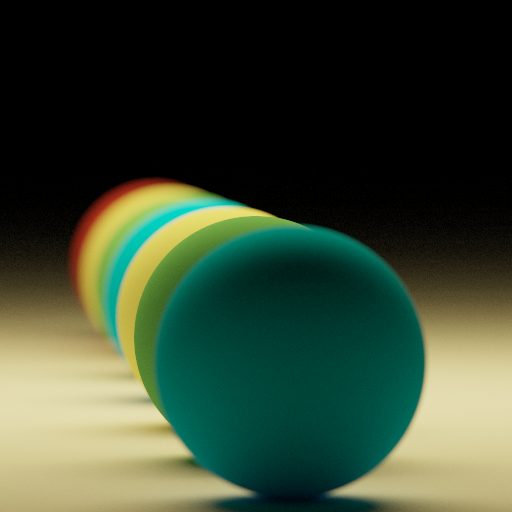
\includegraphics[width=0.65\textwidth]{../img/dof.png}
    \end{center}
\end{frame}

\begin{frame}
    \vfill
    \centering
    \begin{beamercolorbox}[sep=8pt,center,shadow=true,rounded=true]{title}
        \usebeamerfont{title}Demo\par
    \end{beamercolorbox}
    \vfill
\end{frame}

\end{document}
